\chapter{Sensors and Modules}

\section{Sensors}

\subsection{DHT11/DHT22 Sensor}
DHT11/DHT22 sensor is used to measure the temperature and humidity. These sensors contain a chip that does analog to digital conversion and spits out a digital signal with the temperature and humidity.

\begin{minipage}[T]{0.48\linewidth}
   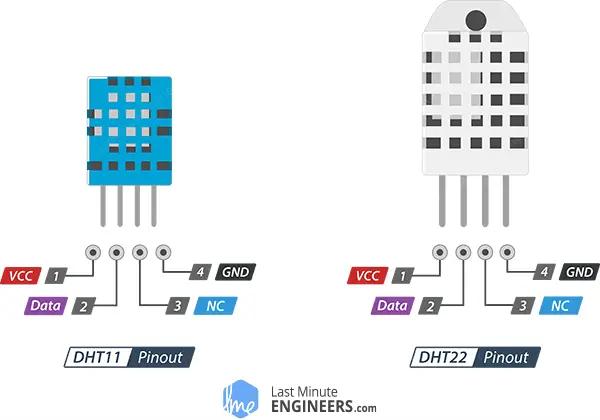
\includegraphics[width=\linewidth]{figures/DHT.png}
\end{minipage}\hfill
\begin{minipage}[T]{0.3\linewidth}
   \begin{tabular}{l}
      \renewcommand{\arraystretch}{1.25}
      \textbf{Logical Code} \\
      \code{dht.\rgbV{readHumidity()}} \\
      \code{dht.\rgbV{readTemperature()}} \\
      \code{dht.\rgbV{readTemperature(\rgbR{true})}} \\
   \end{tabular}
\end{minipage}


\subsection{BMP180 Barometric Sensor}
BMP180 Barometric Sensor measures the absolute pressure of the air around it. It has a measuring range from 300hPa to 1100hPa with an accuracy down to 0.02hPa. It can also measure altitude and temperature.

\begin{minipage}{0.48\linewidth}
   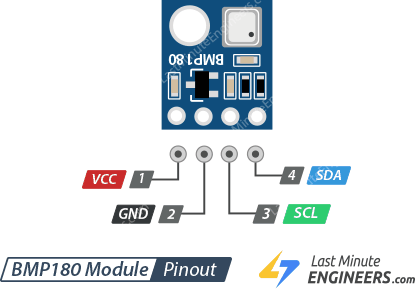
\includegraphics[width=0.8\linewidth]{figures/BMP.png}
\end{minipage}\hfill
\begin{minipage}{0.3\linewidth}
   \begin{tabular}{l}
      \renewcommand{\arraystretch}{1.25}
      \textbf{Logical Code} \\
      \code{bmp.\rgbV{readTemperature()}} \\
      \code{bmp.\rgbV{readPressure()}} \\
      \code{bmp.\rgbV{readAltitude()}}
   \end{tabular}
\end{minipage}


\subsection{Rain Sensor}
The rain sensor is used to detect water and it can detect beyond what a humidity sensor can. \textbf{Wet}: the resistance increases, and the output voltage decreases and \textbf{Dry}: the resistance is lower, and the output voltage is higher.

\begin{minipage}{0.48\linewidth}
   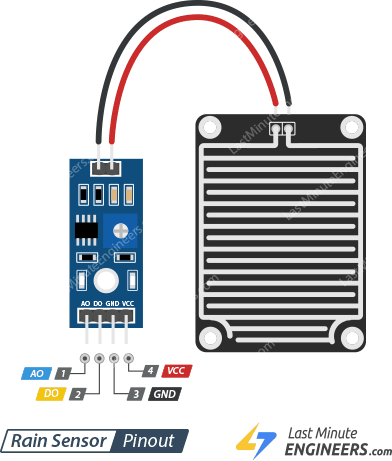
\includegraphics[width=0.8\linewidth]{figures/RAIN.png}
\end{minipage}\hfill
\begin{minipage}{0.3\linewidth}
   \begin{tabular}{l}
      \renewcommand{\arraystretch}{1.25}
      \textbf{Logical Code} \\
      \code{\rgbV{digitalRead(\rgbR{rainPin})}} $\to$ \code{int}\\
      \code{\rgbV{analogRead(\rgbR{rainPin})}} $\to$ \code{int} \\
   \end{tabular}
\end{minipage}


\subsection{Soil Moisture Sensor}
The soil moisture sensor or the hygrometer is usually used to detect the humidity of the soil. So, it is perfect to build an automatic watering system or to monitor the soil moisture of your plants.

\begin{minipage}{0.48\linewidth}
   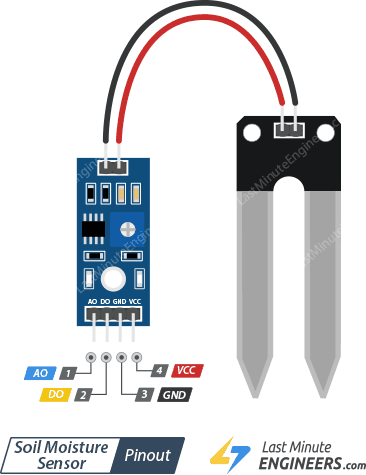
\includegraphics[width=0.8\linewidth]{figures/Soil Moisture.png}
\end{minipage}\hfill
\begin{minipage}{0.3\linewidth}
   \begin{tabular}{l}
      \renewcommand{\arraystretch}{1.25}
      \textbf{Logical Code} \\
      \code{\rgbV{digitalRead(\rgbR{PIN})}} $\to$ \code{int}\\
      \code{\rgbV{analogRead(\rgbR{PIN})}} $\to$ \code{int} \\
   \end{tabular}
\end{minipage}

\pagebreak
\subsection{Gas/Smoke Sensor}
The MQ-2 smoke sensor is sensitive to smoke and to the following flammable gases: LPG, butane, propane, methane, alcohol and hydrogen. The resistance across the sensor is different depending on the type of the gas. The greater the gas concentration, the greater the output voltage.

\begin{minipage}{0.48\linewidth}
   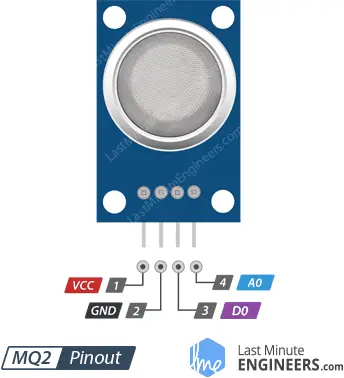
\includegraphics[width=0.8\linewidth]{figures/Gas Sensor.png}
\end{minipage}\hfill
\begin{minipage}{0.3\linewidth}
   \begin{tabular}{l}
      \renewcommand{\arraystretch}{1.25}
      \textbf{Logical Code} \\
      \code{\rgbV{digitalRead(\rgbR{PIN})}} $\to$ \code{int}\\
      \code{\rgbV{analogRead(\rgbR{PIN})}} $\to$ \code{int} \\
   \end{tabular}
\end{minipage}


\subsection{Ultrasonic Sensor}
The HC-SR04 ultrasonic sensor uses sonar to determine distance. It offers excellent non-contact range detection with high accuracy and stable readings in an easy-to-use package. From 2 cm to 400 cm or 1” to 13 feet.

\begin{minipage}{0.48\linewidth}
   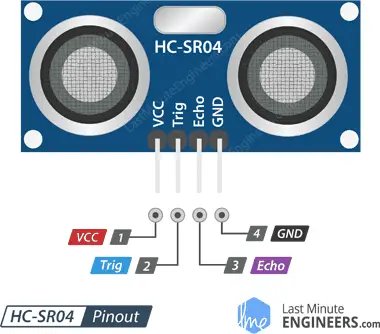
\includegraphics[width=0.8\linewidth]{figures/Ultrasonic Sensor.png}
\end{minipage}\hfill
\begin{minipage}{0.4\linewidth}
   \begin{tabular}{l}
      \renewcommand{\arraystretch}{1.25}
      \textbf{Logical Code} \\
      \code{digitalWrite(\rgbR{trigPin}, \rgbB{LOW})}\\
      \code{delayMicroseconds(\rgbB{2})}\\
      \code{digitalWrite(\rgbR{trigPin}, \rgbB{HIGH})}\\
      \code{delayMicroseconds(\rgbB{10})}\\
      \code{digitalWrite(\rgbR{trigPin}, \rgbB{LOW})}\\
      \code{\rgbO{long} duration = \rgbV{pulseIn(\rgbR{echoPin}, \rgbR{HIGH})}}\\
      \code{cm = (duration/2) / 29.1}\\
      \code{inches = (duration/2) / 74}
   \end{tabular}
\end{minipage}


\pagebreak
\subsection{PIR Motion Sensor}
The PIR motion sensor is ideal to detect movement. PIR stand for “Passive Infrared”. Basically, the PIR motion sensor measures infrared light from objects in its field of view. So, it can detect motion based on changes in infrared light in the environment.

\begin{minipage}{0.48\linewidth}
   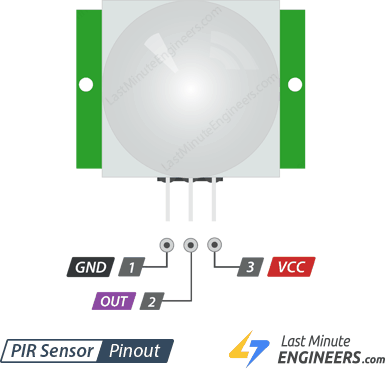
\includegraphics[width=0.8\linewidth]{figures/PIR Sensor.png}
\end{minipage}\hfill
\begin{minipage}{0.35\linewidth}
   \begin{tabular}{l}
      \renewcommand{\arraystretch}{1.25}
      \textbf{Logical Code} \\
      \code{\rgbV{digitalRead(\rgbR{PIN})}} $\to$ \code{HIGH/LOW}
      \\[1ex]
      ** Check \rgbR{state change} using \textbf{if-else} \& \\[-1ex]
      \textbf{save} the current state
   \end{tabular}
\end{minipage}



\subsection{RFID}
RFID means radio-frequency identification. RFID uses electromagnetic fields to transfer data over short distances. Each tag has his own unique identification (UID). Two-way radio transmitter-receiver, the reader, that send a signal to the tag and read its response.

\begin{center}
   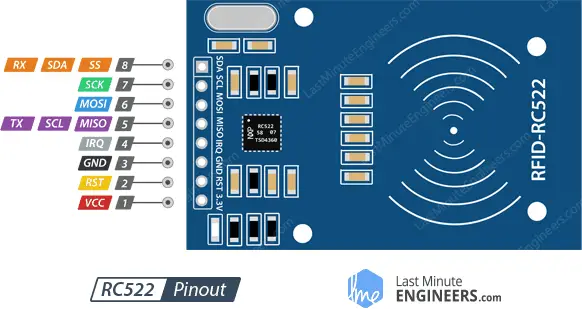
\includegraphics[width=0.6\linewidth]{figures/RFID.png}
\end{center}

\vspace{2ex}
\begin{cpp}
byte authorizedUID[] = {0xAB, 0xCD, 0xEF, 0x12};

bool checkAccess() {
    if (!mfrc522.PICC_IsNewCardPresent() || !mfrc522.PICC_ReadCardSerial()) {
        return false;
    }
    for (byte i = 0; i < mfrc522.uid.size; i++) {
        if (mfrc522.uid.uidByte[i] != authorizedUID[i]) {
            return false;
        }
    }
    return true;
}
\end{cpp}

\pagebreak
\subsection{Microprocessor Sound Sensor}
Microprocessor sound sensor gives a measurement of how loud a sound is.

\begin{minipage}{0.48\linewidth}
   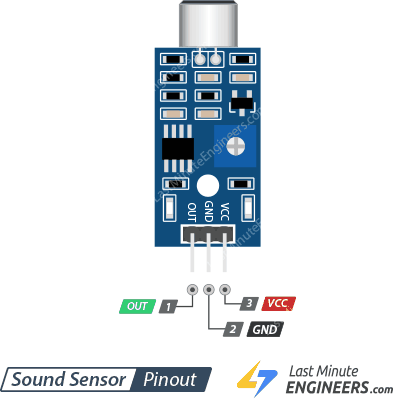
\includegraphics[width=0.8\linewidth]{figures/Sound Sensor.png}
\end{minipage}\hfill
\begin{minipage}{0.35\linewidth}
   \begin{tabular}{l}
      \renewcommand{\arraystretch}{1.25}
      \textbf{Logical Code} \\
      \code{\rgbV{digitalRead(\rgbR{PIN})}} $\to$ \code{int}\\
   \end{tabular}
\end{minipage}


\subsection{Relay Module}
A relay is an electrically operated switch of mains voltage. It can be turned on or off, letting the current go through or not.

\begin{minipage}{0.48\linewidth}
   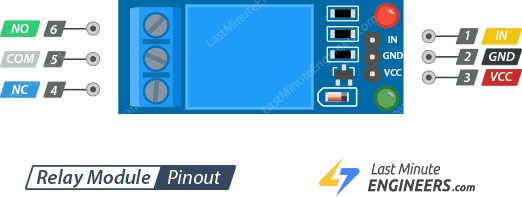
\includegraphics[width=\linewidth]{figures/Relay.png}
\end{minipage}\hfill
\begin{minipage}{0.35\linewidth}
   \begin{tabular}{l}
      \renewcommand{\arraystretch}{1.25}
      \textbf{Logical Code} \\
      \code{digitalWrite(\rgbR{relayPIN}, \rgbB{HIGH/LOW})}\\
   \end{tabular}
\end{minipage}


\subsection{L298N Motor Driver}
The L298N 4WD Motor Driver is a versatile and robust H-bridge driver module designed for controlling DC motors with ease and precision.

\begin{minipage}{0.48\linewidth}
   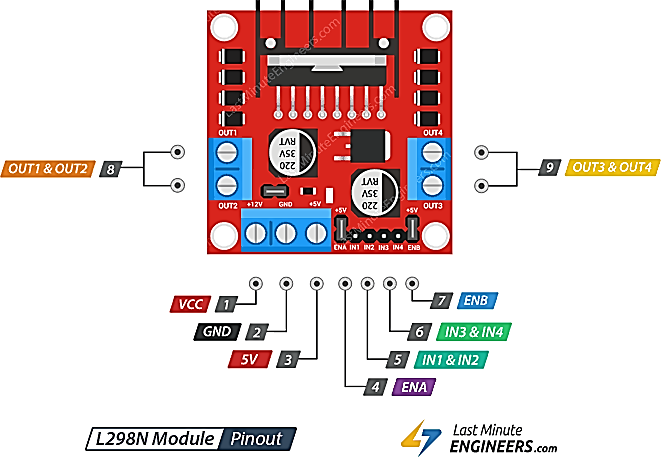
\includegraphics[width=\linewidth]{figures/Motor Driver.png}
\end{minipage}\hfill
\begin{minipage}{0.35\linewidth}
   \begin{tabular}{l}
      \renewcommand{\arraystretch}{1.25}
      \textbf{Logical Code} \\
      \code{digitalWrite(\rgbR{in1}, \rgbB{HIGH})} $\to$ direction\\
      \code{digitalWrite(\rgbR{in2}, \rgbB{LOW})} $\to$ direction\\
      \code{analogWrite(\rgbR{enA}, \rgbB{0-255})} $\to$ speed\\[2ex]
      {HIGH + LOW = Forward} \\
      {LOW + HIGH = Backward} \\
   \end{tabular}
\end{minipage}


\pagebreak
\begin{minipage}{0.45\linewidth}
   \subsection{Servo Motor}
   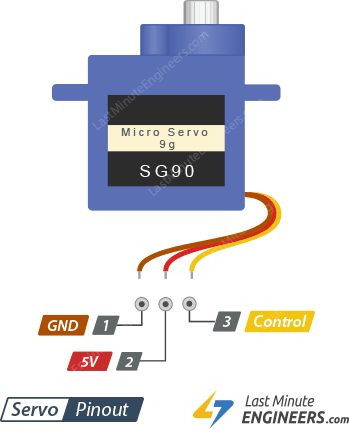
\includegraphics[width=0.55\linewidth]{figures/Servo.png}
   
   \vspace{2ex}
   \begin{tabular}{l}
      \renewcommand{\arraystretch}{1.25}
      \code{myServo.\rgbV{write}(0-180)}\\
   \end{tabular}
\end{minipage}\hfill
\begin{minipage}{0.51\linewidth}
   \subsection{Bluetooth Sensor}
   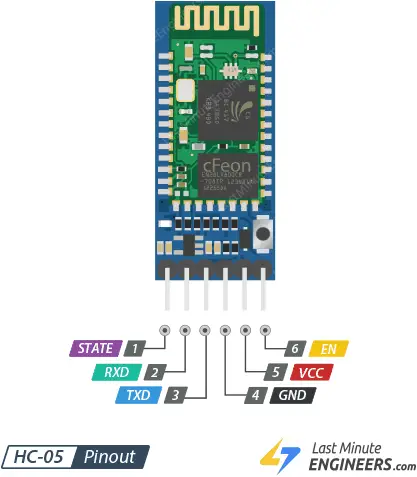
\includegraphics[width=0.55\linewidth]{figures/Bluetooth.png}
   
   \vspace{2ex}
   \begin{tabular}{l}
      \renewcommand{\arraystretch}{1.25}
      \code{bluetoothSerial.\rgbV{available}() | \rgbV{read()} | \rgbV{write()}}\\
   \end{tabular}
\end{minipage}



\subsection{IR Sensor}
\begin{minipage}{0.48\linewidth}
   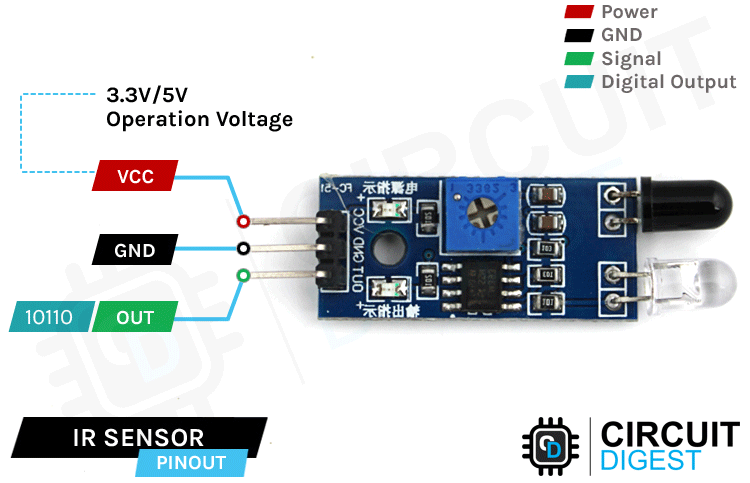
\includegraphics[width=\linewidth]{figures/IR.png}
\end{minipage}\hfill
\begin{minipage}{0.42\linewidth}
   \begin{tabular}{l}
      \renewcommand{\arraystretch}{1.25}
      \textbf{Logical Code} \\
      \code{\rgbO{int} irValue = \rgbV{digitalRead(\rgbR{irPin})}}\\[2ex]
      \code{if (irValue == HIGH)\{}\\
      \code{   Serial.println("No Obstacle Detected");}\\
      \code{\} else \{}\\
      \code{   Serial.println("Obstacle Detected");}\\
      \code{\}}
   \end{tabular}
\end{minipage}


\subsection{Water Level Sensor}

\begin{minipage}{0.48\linewidth}
   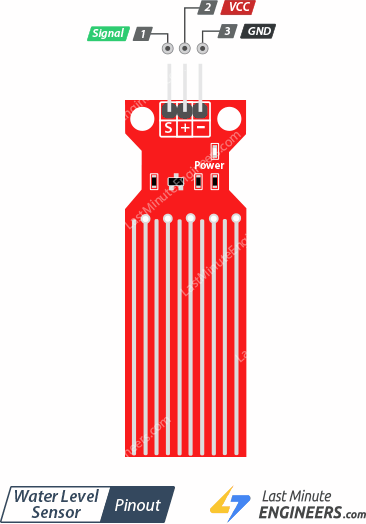
\includegraphics[width=0.7\linewidth]{figures/Water Level.png}
\end{minipage}\hfill
\begin{minipage}{0.42\linewidth}
   \begin{tabular}{l}
      \renewcommand{\arraystretch}{1.25}
      \textbf{Logical Code} \\
      \code{\rgbO{int} waterLevel = \rgbV{analogRead(\rgbR{PIN})}}\\[2ex]
      Outputs: \rgbO{0 to 1023}\\
      Higher values indicate more water.
   \end{tabular}
\end{minipage}


\subsection{Arduino Uno}

\vspace{6ex}
\begin{center}
   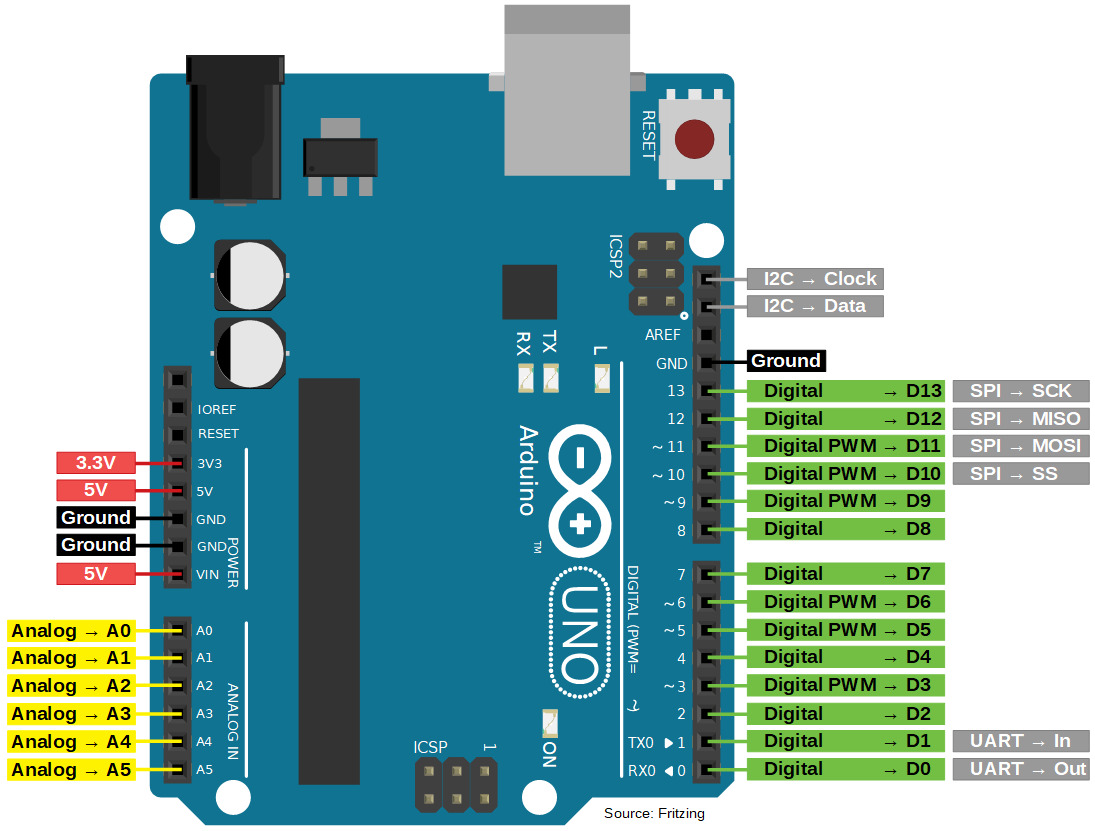
\includegraphics[width=0.8\linewidth]{figures/Arduino.png}
\end{center}

\vspace{6ex}
\begin{center}
   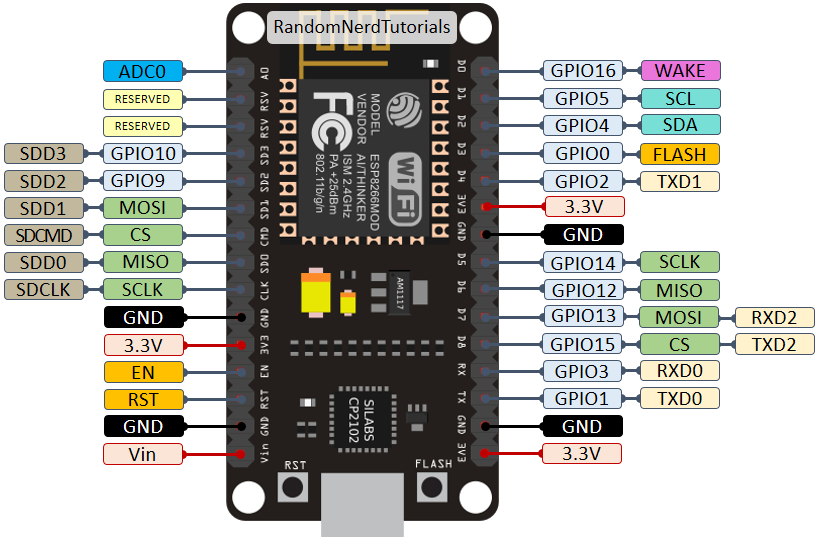
\includegraphics[width=0.8\linewidth]{figures/ESP8266.png}
\end{center}